\documentclass[a4paper,12pt]{scrreprt}

% --- Encoding / Sprache / Fonts ---
\usepackage[utf8]{inputenc}
\usepackage[T1]{fontenc}
\usepackage[english]{babel}
\usepackage{microtype}
\usepackage{xurl}
\setlength{\emergencystretch}{3em}
\usepackage{lmodern}
% \usepackage{microtype}
\usepackage{csquotes}

% --- Layout ---
\usepackage{geometry}
\geometry{
    a4paper,
    left=2.5cm,
    right=2.5cm,
    top=2.5cm,
    bottom=2.5cm,
}
\usepackage{setspace}
\onehalfspacing
% \setlength{\parindent}{0pt} % für Zeileneinzug bei Paragraphen

% --- Grafiken / Tabellen ---
\usepackage{graphicx}
\usepackage{booktabs}
\usepackage{array}
\usepackage{longtable}
\usepackage{makecell}
\usepackage{float}
\usepackage{rotating}
\usepackage[table]{xcolor}

% --- Mathe ---
\usepackage{amsmath,amsfonts,amssymb}
\numberwithin{equation}{section}

% --- Listings / Code ---
\usepackage{listings}
\usepackage{verbatim}
\usepackage{caption}
\captionsetup{justification=centering}
\renewcommand{\lstlistingname}{Text-Abbildung}
\lstset{
    basicstyle=\ttfamily,
    numbers=left,
    numberstyle=\tiny,
    stepnumber=1,
    showstringspaces=false,
    frame=single,
    captionpos=b,
    breaklines=true,
}

\usepackage{subcaption}
\usepackage{tikz}
\usetikzlibrary{shapes.geometric, arrows.meta, positioning}
\tikzset{
    block/.style = {rectangle, draw=black, minimum width=2.8cm, minimum height=0.8cm, text centered, rounded corners},
    arrow/.style = {-{Stealth}, thick}
}
\usepackage{algorithm}
\usepackage{algorithmic}
\usepackage{enumitem}
\usepackage{dirtytalk}
\usepackage{indentfirst}
\usepackage{siunitx}
\usepackage{url}

% --- PDF / Anhang ---
\usepackage{pdfpages}

% --- Header/Footer ---
% \usepackage{fancyhdr}
% \pagestyle{fancy}
% \fancyhf{}
% \fancyhead[L]{Bachelorarbeit}
% \fancyhead[R]{\leftmark}
% \fancyfoot[C]{\thepage}

\usepackage[automark]{scrlayer-scrpage}
\clearpairofpagestyles

\ihead{Master's thesis}
\ohead{\headmark}
\cfoot{\pagemark}

\pagestyle{scrheadings}
\renewcommand*\chapterpagestyle{scrheadings}
\renewcommand{\bibname}{References}

\KOMAoptions{headsepline=true}

% --- Links / Referenzen (Reihenfolge beachten) ---
\usepackage{hyperref}
\usepackage{cleveref}

% --- Glossar + Abkürzungen (statt glossaries) ---
\usepackage[nomain,acronym,nonumberlist,automake]{glossaries-extra}
\setabbreviationstyle[acronym]{long-short}
\makeglossaries

% --- Frontmatter/Mainmatter/Backmatter (wie Kollege) ---
\makeatletter
\newcommand{\frontmatter}{
    \cleardoublepage
    \pagenumbering{Roman}
    \setcounter{page}{1}
}
\newcommand{\mainmatter}{
    \cleardoublepage
    \pagenumbering{arabic}
    \setcounter{page}{1}
}
\newcommand{\backmatter}{
    \cleardoublepage
    \pagenumbering{Roman}
}
\makeatother

% --- Meta ---
\title{Some Title to be inserted right here}
\author{Max Mustermann}
\date{\today}

\begin{document}

%TC:ignore
% Deine Glossar-/Acronym-Definitionen (sollte \newacronym und \newglossaryentry enthalten)
    \newglossaryentry{ui}{
    name=UI,
    description={User Interface}
}

\newglossaryentry{ux}{
    name=UX,
    description={User Experience}
}

\newglossaryentry{llm}{
    name=LLM,
    description={Large Language Model}
}

\newglossaryentry{dom}{
    name=DOM,
    description={Document Object Model}
}

\newglossaryentry{json}{
    name=JSON,
    description={JavaScript Object Notation}
}

\newglossaryentry{http}{
    name=HTTP,
    description={HyperText Transfer Protocol}
}

% Dies ist ein Test-Kommentar, um zu schauen, ob das Backup funktioniert

    \begin{titlepage}
        \centering

        \begin{flushleft}
            \includegraphics[
                height=1.5cm,
                keepaspectratio
            ]{/path/to/your/logo)}
        \end{flushleft}

        \vspace{1cm}

        {\LARGE \textbf{\textsf{<INSERT YOUR TITLE HERE>}}} \\[0.8cm]

        \textbf{Author: } \\
        Max Mustermann \\[0.5em]

        \textbf{Student ID no: } \\
        <STUDENT ID NO HERE> \\[0.8cm]

        \textbf{University: } \\
        <UNIVERSITY HERE> \\[0.5em]

        \textbf{Faculty: } \\
        <FACULTY HERE> \\[0.8cm]

        \textbf{First examiner: } \\
        <NAME FIRST EXAMINER HERE> \\[0.5em]

        \textbf{Second examiner:} \\
        <NAME SECOND EXAMINER HERE> \\[0.8cm]

        \textbf{Course of studies:} \\
        <COURSE OF STUDIES HERE> \\[0.8cm]

        \textbf{Project type:} \\
        <PROJECT TYPE HERE> \\[0.8cm]

        \textbf{Semester:} \\
        <SEMESTER HERE> \\[0.8cm]

        \textbf{Submission date:} \\
        \today

    \end{titlepage}



% \includepdf[pages=-]{src/eigenstaendigkeitserklaerung_printed.pdf}

% --- Verzeichnisse (Frontmatter) ---
    \frontmatter
    \tableofcontents


    \cleardoublepage

    \listoffigures
    \cleardoublepage

    \listoftables
    \cleardoublepage

% Abkürzungsverzeichnis (nur wenn du \newacronym nutzt)
    \printglossary[type=\acronymtype, title={List of abbreviations}]
    \cleardoublepage

%TC:endignore

% --- Inhalt (Mainmatter) ---
    \mainmatter
    \chapter{Einleitung}\label{ch:einleitung}

\lipsum

    \chapter{Grundlagen}\label{ch:grundlagen2}

\section{Beispiel-Zitat}\label{sec:beispiel-zitat}

Dies ist ein Beispiel-Zitat\cite{owasp-top10}.
Du kannst schreiben, was in dieser Quelle erwähnt wurde,
kannst den Zitier-Befehl im vorherigen Satz schreiben und das Zitat erscheint in dem gewählten Zitierstil und
ist ebenfalls im Literaturverzeichnis zu sehen.

\section{Beispiel-Abbildung}\label{sec:beispiel-abbildung}

Dies ist eine Beispiel-Abbildung.
Diese Abbildung kannst du mit dem Befehl hier Referenzieren: \cref{fig:anylabel}:

\begin{figure}[h!]
	\centering
	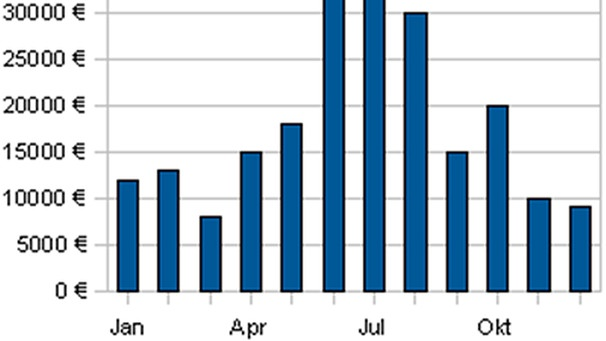
\includegraphics[width=\textwidth]{src/assets/some_graph}
	\caption{Einbinden einer Beispiel-Grafik}
	\label{fig:anylabel}
\end{figure}

Die Grafiken werden automatisch nummeriert, brauchen jedoch ein eindeutig identifizierbares Label, um
solche Grafiken referenzieren zu können.

\section{Beispiel-Code}\label{sec:beispiel-code}

\section{Beispiel-Tabelle}\label{sec:beispiel-Tabelle}

\section{Beispiel-Glossar-Referenzen}\label{sec:glossar-referenz}
    \chapter{Konzept}\label{ch:konzept}

\lipsum


    \chapter{Implementierung}\label{ch:implementierung}

\lipsum
    \chapter{Evaluierung}\label{ch:evaluierung}

\lipsum
    \chapter{Fazit und Ausblick}\label{ch:fazit-und-ausblick}

\lipsum

% --- Literatur + Backmatter ---

%TC:ignore
    \backmatter


    \bibliographystyle{ieeetr}
    \bibliography{main}

    \chapter*{Overview of tools used}\label{ch:liste-genutzter-hilfsmittel}

%TC:endignore

\end{document}